\documentclass[preview]{standalone}

\usepackage{amsmath}
\usepackage{amssymb}
\usepackage{stellar}
\usepackage{bettelini}

\hypersetup{
    colorlinks=true,
    linkcolor=black,
    urlcolor=blue,
    pdftitle={Biologia},
    pdfpagemode=FullScreen,
}

\begin{document}

\title{Biologia}
\id{biologia-riflesso-patellare}
\genpage

\begin{snippetdefinition}{riflesso-patellare-definition}{Riflesso patellare}
    Il \textit{riflesso patellare} è il riflesso spontaneo prodotto
    da uno stimolo sul ginocchio.
\end{snippetdefinition}

\begin{snippet}{patellare-illustration}
    \begin{center}
    \begin{figure}[ht]
        \centering
        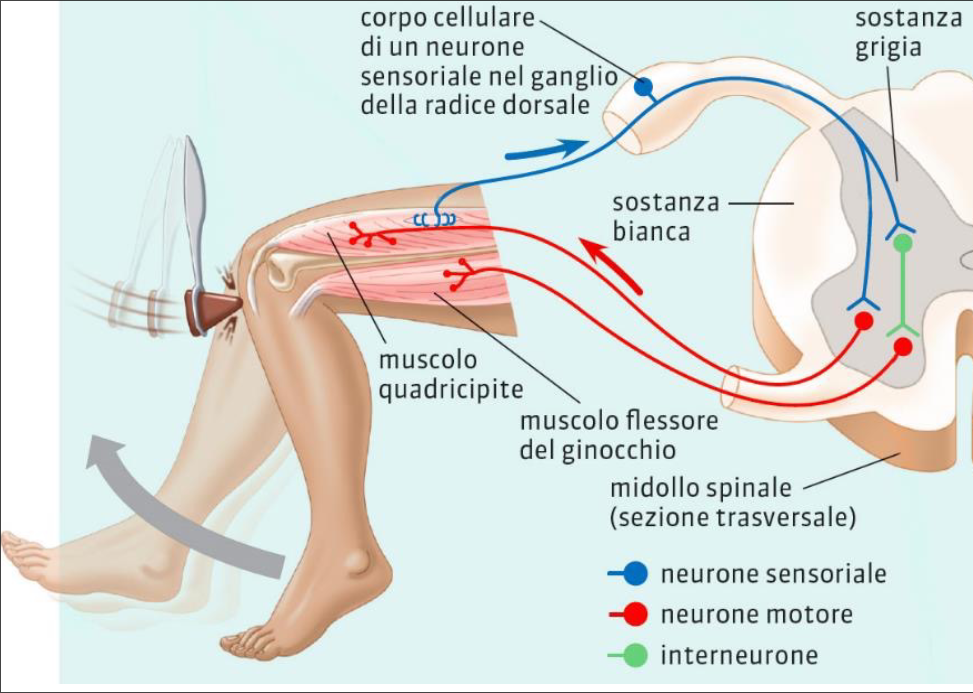
\includegraphics[width=0.75\textwidth]{./resources/patellare.png}
    \end{figure}
    \end{center}
\end{snippet}

\end{document}